\clearpage
\section{Background estimation for processes with genuine \texorpdfstring{\met}{MET}\label{sec:backgrounds}}

After applying the full hadronic selection, the remaining backgrounds are SM
processes with genuine \met in the final state. In the category of zero b-tagged 
jets, the two primary background are:
\begin{itemize}
\item \zj; where the Z vector boson decays into a pair of neutrinos, 
\item \wj; where the W vector boson either undergoes a leptonic decay and the lepton is ``lost''
or it undergoes the weak decay $\wtaunu$ where the $\tau$ decays into quarks and 
\end{itemize}

a ``lost'' lepton is defined as any lepton that isn't reconstructed or 
fails the isolation or acceptance requirements. Other SM backgrounds, 
such as the diboson production, single-top and Drell-Yan are expected.

for events with one or more b-tagged jets, \ttbar production where each
quark decays into a b-quark and a W vector boson which in turn decays into 
a lost lepton and neutrino becomes a large background source.

%For events with only one reconstructed
%b-quark jet, the contribution of both W + jets and Z + jets
%backgrounds are of a similar size to the \ttbar background.  
For events with two reconstructed b-quark jets, \ttbar production
dominates the background. 

This analysis uses a ``data-driven'' method to estimate backgrounds
in the hadronic signal model. Data control samples are used to predict
background SM yields instead of direct measurement in MC simulations. 
This approach has two benefits, 1. The beam and detector conditions 
for the hadronic and control samples are very similar. 2. The information 
used from MC simulation is in the form of ratios~\ref{sec:background-method}, 
which has the benefit of canceling potential sysetematic effects in simulation.

Two control samples are used to estimate the background. To esimate the
\znunu + jets background, $\gamma$ + jets events, which have the same
kinematic properties as \znunu + jets when the photon is ingored but 
different acceptance. ~\cite{PAS-SUS-08-002,Bern:2011pa}  A \mj control
sample is used to estimated the all remaining background including the 
dominant \wj and \ttbar process.

The following sections describe the estimation method and contol selection.

\subsection{Overview of the method\label{sec:background-method}}

Consider a bin in  \scalht, \njet, \nb, the method predicts the number 
of expected background processes in a signal region ($\npre^{\rm  signal}$) 
by translating from the observed data yield in a control region 
($\nobs^{\rm  control}$) through the use of a {\it translation factor} 
(TF) constructed from the ratio of MC signal and control yields ie:

\begin{equation}
  \label{equ:pred-method}
  \npre^{\rm signal} = \underbrace{\frac{N_{\rm MC}^{\rm
      signal}}{N_{\rm MC}^{\rm
      control}}}_\text{translation factor}\! \times \; \nobs^{\rm
    control}   
\end{equation}

The sum of expected yields from all MC samples, obtained for the
relevant control sample selection, enter the denominator of each
transfer factor:

\begin{equation}
  \label{equ:ratio-denom}
  N_{\rm MC}^{\rm control} = N_{\rm W} + N_{\ttbar} + N_{\znunu} +
N_{\rm DY} + N_{\gamma} + N_{\rm top} + N_{\rm di-boson}
\end{equation}


As described in [REF], depending on the b-tag category, one or both
control samples are used to predict the backgrounds in the signal region.
For the  b-jet multiplicity bins $n_b = 0$ and $n_b = 1$, the \mg and 
\gj control samples are used to predict to total background. The \gj control
sample is used to predict the \znunu + jets background and the expected yield
obtained from the \znunu sample enters the numerator of each transfer
factor:

\begin{equation}
  \label{equ:ratio-numer-gj}
  N_{\rm MC}^{\rm signal}(\scalht,\njet,0 \leq \nb \leq 1) = N_{\znunu}
\end{equation}

for the same \bjet categories, The \mj control sample is used to predict 
the remaining SM background processes, namely the W + jets, \ttbar + jets,
Drell-Yan, di-boson and single top backgrounds, and the total expected yield
from these processes enter the The numerator of each transfer factor:

\begin{equation}
  \label{equ:ratio-numer-mj}
  N_{\rm MC}^{\rm signal}(\scalht,\njet,\nb \leq 1) = N_{\rm W} +
  N_{\ttbar} + N_{\rm DY} + N_{\rm top} + N_{\rm di-boson}
\end{equation}

only the \mj control sample is used to predict the background.
for the b-tag multiplicty bin $n_b = 2$,  The \gj control sample is not 
used as the yields in this data control sample is expected to be low
due to the requirement of at least two b jets per event. The method of
using a W + jets sample to predict the \znunu\ + jets background has
been used previously~\cite{RA1Paper, RA1Paper2011, RA1Paper2012}.  
Therefore the total predicted expected yield from all processes are used 
enter the numerator of each transfer factor:


\begin{equation}
  \label{equ:ratio-numer-mj}
  N_{\rm MC}^{\rm signal}(\scalht,\njet,\nb = 2) = N_{\rm W} +
  N_{\ttbar} + N_{\rm DY} + N_{\rm top} + N_{\rm di-boson} + N_{\znunu}
\end{equation}


The control samples used to predict the SM backgrounds for each 
event category are summarised in Table~\ref{tab:fit-plots}.

This analysis benefits from using translation factos has potential systematic
effects from simulation are expected to cancel out in the translation factor.
The control sample selections are described in the subsequent sections. 

\begin{table}[ht!]
  \caption{Summary of control samples used to predict the SM
    background for each event category. }
  \label{tab:fit-plots}
  \centering
  \begin{tabular}{ lll }
    \hline
    \hline
    \njet   & \nb     & Control samples \\ [1.0ex]
    \hline
    2--3    & 0       & \mj,  \gj  \\
    2--3    & 1       & \mj,  \gj  \\
    2--3    & 2       & \mj        \\
    $\geq$4 & 0       & \mj,  \gj  \\
    $\geq$4 & 1       & \mj,  \gj  \\
    $\geq$4 & 2       & \mj             \\
    \hline
    \hline
  \end{tabular}
\end{table}


%The selection criteria for the three control samples closely resemble
%those for the signal region, differing mainly through the use of a
%muon, di-muon, or photon {\it tag} (that is ignored in the calculation
%of jet-based kinematic variables such as \scalht, \mht, \alphat, \etc)
%and some minimal additional kinematic requirements (\eg invariant or
%transerve mass windows) to obtain W, Z, and \ttbar-enriched event
%samples. The same selection criteria are designed to suppress signal
%contamination in the control samples so that unbiased data-driven
%estimates for the SM backgrounds in the signal region can be
%made. Hence, we refer to these samples as {\it control} samples
%although in the final simultaneous fit, any potential signal
%contamination is properly taken into account.
%
%The control sample definitions and binning scheme are chosen so that
%the reliance on simulation to extrapolate correctly from a control
%region to the signal region is minimised. Many systematic effects are
%expected to cancel largely in the transfer factor. However, a
%systematic uncertainty is assigned to each transfer factor to account
%for theoretical uncertainties and effects such as the mismodelling of
%kinematics (\eg acceptances) and instrumental effects (\eg
%reconstruction efficiencies), as described in
%Sec.~\ref{sec:bkgd-syst}.
%
%%Kinematic cuts are applied to enrich as much as possible the \wj,
%%\ttbar, and \znunu components in the muon and di-muon control
%%samples. The definition of the samples are geared towards efficiency
%%rather than purity (even so, the purities are at the level $>$90\%)
%%and any contamination from "backgrounds" (\eg \ttbar in the case of
%%the \mmj sample) are simply incorporated into the transfer
%%factors. Alternatively, a zero b-jet requirement can be applied to the
%%\mmj sample to obtain a higher purity of Z$\rightarrow\mu\mu$ + jets
%%events (\ie, with reduced contamination from \ttbar), which can then
%%be used to give an expectation for the \znunu + jets background for
%%all b-jet categories in the signal region.
%
\subsection{Definition of the control samples\label{sec:def-control-samples}}

\subsubsection{Muon and photon triggers\label{sec:muon_triggers}}

Events for the muon control sample are recorded with the \verb!HLT_IsoMu24_eta2p1! 
trigger. Figure~\ref{fig:eff-muon} (left) shows the \verb!HLT_IsoMu24_eta2p1! 
trigger efficiency as determined in bins of number of primary vertices 
for muon $\pt >$ 25 \gev and $|\eta| <$ 2.1~\cite{ref:muon-eff}.
Figure~\ref{fig:eff-muon} (right) shows the distribution of the number 
of vertices in the muon control sample seeded by the \verb!HLT_IsoMu24_eta2p1!. 
The efficiency at the mean number of vertices $n_{vtx}=13$ is taken as flat
trigger efficiency across \njet, \nb, and \scalht. This measurement 
agrees well with direct tag and probe measurements in bins of 
\njet, \nb, \scalht done elsewhere~\cite{RA1Paper2012}.

\begin{figure}[!h]
  \begin{center}
  \subfigure{
    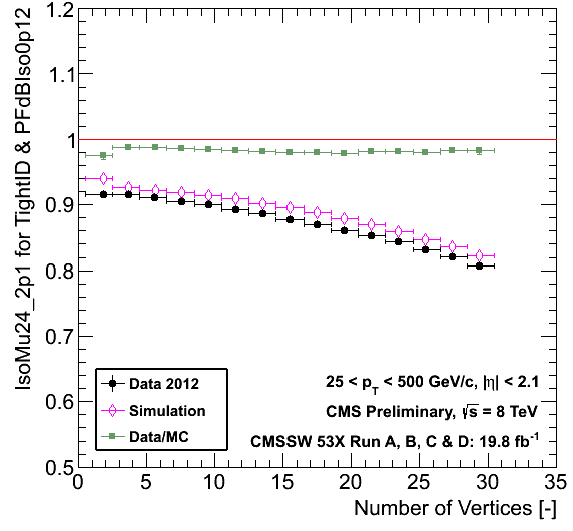
\includegraphics[width=0.3\textwidth,]{figures/trigger/muonEffvsNvtx}
    }   
  \subfigure{
   \includegraphics[width=0.42\textwidth,page=65]{figures/data-mc/v21/mu/muonLook_pfJet_ge2j_375.pdf}
   }\\     
    \caption{\label{fig:eff-muon}
    (left) Muon trigger efficiency as a function of
    number of primary vertices for muon $\pt>$ 25 \gev and
    $|\eta| <$ 2.1. (right) Number of primary vertices
    in muon control sample.} 
 
  \end{center}
\end{figure}

Events for the photon control sample are recorded with the
\verb!HLT_Photon150! trigger, which is $\sim100\%$ efficient for
$E_{\rm T}^{\rm photon} > 165\gev$ and $\scalht > 375\gev$, as shown
in Figure~\ref{fig:eff-photon}. The efficiency measurement is made
using the \verb!HLT_Photon90! trigger as a reference.

\begin{figure}[!h]
  \begin{center}
  \subfigure[\njetlow]{
    \includegraphics[width=0.43\textwidth,page=6]{figures/trigger/g_barrel_375_caloJet_le3j_}
    }   
  \subfigure[\njethigh]{
   \includegraphics[width=0.43\textwidth,page=6]{figures/trigger/g_barrel_375_caloJet_ge4j_}
   }\\     
    \caption{\label{fig:eff-photon}
    Cumulative efficiency turn-on curves for the \texttt{HLT\_Photon150} trigger 
    as a function of photon \pt for events satisfying \njetlow 
    (left) and \njethigh (right).} 
  \end{center}
\end{figure}

\FloatBarrier


\subsubsection{The \texorpdfstring{\mj}{muon plus jets} control sample}
%
\wj and \ttbar processes are found in the hadronic signal region 
when the decay lepton is missed by the lepton veto, either 
because it was not reconstructed properly, fell out of acceptance 
or alternatlively, decayed hadronically in the case of a tau lepton 
from a high-p$_{T}$ W boson. Instead of directly relying on MC 
simulation to estimate these background, a \mj control sample is 
used where the selection criteria is chosen to identify W bosons 
decaying to a muon and a neutrino. Then by removing the muon from 
the event, one effectively selects a sample of W boson decaying to 
a neutrino and a lost lepton. The muon is not considered in the 
calculation of \scalht, \mht, or \alphat and cuts on such jet-based 
quantities are kept consistent with those applied in the hadronic 
search region with the only exception being that no \alphat requirement 
is made, as motivated by the discussion in Sec.~\ref{sec:larger}. 

In order to select events containing W bosons, exactly one tight 
isolated muon~\ref{sec:reconstruction} within an acceptance of 
\PT $>$ 30 \gev and $|\eta| <$ 2.1 is required, and the
transverse mass of the W candidate, 
$M_{T} = \sqrt{2\pt^{\mu}\met(1-cos(\Delta\phi(\vec{\pt}^{\mu},\met))}$ 
must between 30 and 125~\gev. This latter helps suppress QCD multijet 
and potential signal events. Events are vetoed if a muon is found inside
the radius of a jet, i.e. $\Delta R(\mu,\textrm{jet}) < 0.5$.
The single isolated track veto, described in sections~\ref{sec:reconstruction} 
and~\ref{sec:vetoes}, is also applied, which considers all 
single isolated tracks in the event except that associated with 
the identified, isolated muon. Lastly, the cleaning cut the cleaning cut 
$\mht/\pfmet$ described in ~\ref{sec:finalSelection} is also applied, 
where the \pfmet is adjusted to account for the transverse momentum of the 
identified, isolated muon.

%\subsubsection{The \texorpdfstring{\mmj}{di-muon plus jets} control sample}
%
%The \znunu\ + jets process forms an irreducible background and can be
%estimated using the \zmumu + jets process, which has similar kinematic
%properties but a different acceptance and a smaller branching ratio. A
%background estimate is obtained through the use of a \mmj sample. Most
%of the selection criteria are identical to those for the \mj sample,
%but the few that differ are tuned to identify Z bosons decaying to two
%muons in the kinematic phase space of the signal region. The muons are
%not considered in the calculation of event-level variables such as
%\scalht, \mht and \alphat. All cuts on such jet-based quantities are
%consistent with those applied in the hadronic search region and the
%same \njet, \nb, and \scalht binning is used. The only exception is
%that no \alphat requirement is made, as motivated by the discussion in
%Sec.~\ref{sec:larger}. In order to select an event sample containing Z
%bosons, exactly two tight isolated muons within an acceptance of $\Pt
%> 30\gev$ and $|\eta| < 2.1$ are required (due to the trigger). The
%invariant mass of the two muons must satisfy $m_{Z} - 25 <
%M_{\mu_1\mu_2} < m_{Z} + 25$. Events are vetoed if $\Delta
%R(\mu_{i},\textrm{jet}_j) < 0.5$ is satisfied, running over all muons
%$i$ and all jets $j$. The single isolated track veto, described in
%Sections~\ref{sec:reconstruction} and~\ref{sec:vetoes}, is also
%applied, considering all single isolated tracks in the event except
%those associated with the two identified, isolated muons. Finally, the
%cleaning cut $\mht/\pfmet$ is also applied, as done in the signal
%region, where the \pfmet is adjusted to account for the transverse
%momenta of the two identified, isolated muons. The \mmj sample can be
%used to make predictions in all the \scalht bins, providing coverage
%at low \scalht where the \gj sample cannot.

\subsubsection{The \texorpdfstring{\gj}{photon plus jets} control sample}

The \znunu + jets background is estimated using \gj events which
have a higer cross-section but similar kinematic properties as 
\znunu + jets when the photon is ignored~\cite{PAS-SUS-08-002,Bern:2011pa}. 
The \gj sample is obtained by requiring exactly one tightly 
identified and isolated photon (as defined in section~\ref{sec:reconstruction})
with a transverse momentum of at least 165\gev. The photon is required to be contained 
within the barrel of the detector, ie $|\eta| <1.44$. and to not overlap with 
any reconstructed jets ($\Delta R(\gamma,\textrm{jet}) < 1.0$.)
All other selections are consistant with the hadronic search region
including the \alphat>0.55 cut.

%\subsection{Increasing the acceptance of the muon control samples\label{sec:larger}}
%
%As described in Sec.~\ref{sec:def-control-samples} above, the
%selection criteria of the three control samples are defined such that
%the background composition and event kinematics of the three control
%samples mirror as closely as possible those for the signal
%region. This is done in order to minimise the reliance on the
%simulation to model correctly the backgrounds and event kinematics in
%the control and signal samples.
%
%However, in the case of the \mj and \mmj samples, no requirement is
%made on \alphat in the selection criteria of the samples. This is made
%possible by the remaining kinematic selection criteria, which are
%sufficiently selective to ensure that the muon samples remain rich in
%events from the \wj, \ttbar and \zmumu processes with negligible
%contamination from QCD multijet events. These selection criteria
%include, for example, requiring exactly one or two tight isolated
%muon(s), and imposing acceptance windows on the invariant mass of the
%di-muon sytem or the transverse mass of the muon-\pfmet system, as
%described above. 
%%The absence of QCD multijet events is demonstrated by the control
%%distributions shown in Sec.~\ref{sec:est-control-samples} below. 
%Thus, the acceptance of the two muon control samples can be
%significantly increased, which simultaneously improves their
%predictive power and further reduces the effect of any potential
%signal contamination.  In the case of the \gj sample (used only for
%the region $\scalht > 375\gev$), the requirement $\alphat > 0.55$ is
%still necessary to suppress contamination from QCD multijet events,
%even after the substantial photon \pt cut in the offline selection.
%
%The extrapolation in the variable \alphat is tested through a
%dedicated set of closure tests, described in Sec.~\ref{sec:bkgd-syst},
%which demonstrate that the different \alphat requirements for the \mj
%and \mmj control samples and signal region have no significant
%systematic bias on the prediction. That the \alphat variable
%introduces no acceptance bias for processes with genuine \met is due
%to the accurate modelling by the CMS simulation of such processes,
%namely W + jets, \ttbar, and \znunu\ + jets. Background estimates for
%these processes are provided by the \mj and \mmj samples, as
%identified at the beginning of this Section. Importantly, the same
%cannot be said for QCD multijet events, as in this case the only
%events that survive the \alphat cut are pathological cases in which a
%jet is severely mismeasured or even lost due to detector
%inefficiencies. Such effects certainly do change the event kinematics
%and, in these cases, an \alphat cut will selectively choose events
%with particular kinematic features and topologies. For these
%pathological cases, one cannot rely on MC to model correctly the
%behaviour and therefore the \alphat acceptance. This is a crucial
%distinction to be made between QCD multijet events and processes with
%significant genuine \met. The assumption is that processes with
%genuine \met are selected by the \alphat variable based on the
%escaping invisible particle(s) rather than any pathological effects.
%
%%\subsection{Distributions from the data control samples\label{sec:est-control-samples}}
%%
%%Distributions of key variables for the \mj, \mmj, and \gj samples are
%%shown in below in Figs.~\ref{fig:mu-distr}, \ref{fig:mumu-distr},
%%and~\ref{fig:phot-distr}, respectively. The first two figures show
%%the (leading) muon \pt and isolation distributions, along with the
%%leading jet \pt, \scalht, \mht and \alphat distributions. For the \gj
%%sample, the photon \pt distribution is%and isolation distributions are
%%shown in place of the corresponding muon distribution.%s.
%%No requirement is made on the number of b-jets per event. In general,
%%the agreement between data and simulation is good, giving confidence
%%that the samples are well understood. The MC distributions highlight
%%the composition of each sample. The contribution from QCD multijet
%%events is expected to be negligible.
%%
%%Figure~\ref{fig:jet-bjet} shows the jet and b-jet multiplicity
%%distributions for the \mj, \mmj, and \gj control samples, as defined
%%in Sec.~\ref{sec:def-control-samples} and following the requirement
%%$\scalht > 375\gev$. An accurate modelling of the jet multiplicity in
%%data is achieved for all samples. The b-jet distributions demonstrate
%%the changing background composition as a function of the number of
%%b-jets. For the \mj and \mmj samples, the requirement of zero b-jets
%%results in sub-samples that are rich in W and Z bosons, respectively,
%%with little contamination from \ttbar. The \ttbar background becomes
%%dominant in the \mj sample when exactly one b-jet is required. The
%%requirement of up to two b-tags per event significantly suppresses all
%%processes except for \ttbar production. Requiring at least three
%%b-tags also suppresses \ttbar production. In the case of the \mmj
%%sample, some contamination from \ttbar is observed for $\nb =
%%1$. Requiring more than one b-jet significantly suppresses the yields
%%in both the \mmj and \gj samples.
%%
%%\clearpage
%%\begin{figure}[!h]
%%  \centering
%%  \subfigure[Muon \pt.]{
%%    \includegraphics[width=0.4\textwidth]{figures/data-mc/v1/muon/Stack_muPt_Muon_all_OneMuon_-1To-2b_log}
%%  } 
%%  \subfigure[Muon isolation.]{
%%    \includegraphics[width=0.4\textwidth]{figures/data-mc/v1/muon/Stack_muonIso_Muon_all_OneMuon_-1To-2b_log}
%%  } \\
%%  \subfigure[Transverse mass.]{
%%    \includegraphics[width=0.4\textwidth]{figures/data-mc/v1/muon/Stack_PFMTmu_Muon_all_OneMuon_-1To-2b_log}
%%  } 
%%  \subfigure[\scalht.]{
%%    \includegraphics[width=0.4\textwidth]{figures/data-mc/v1/muon/Stack_HT_Muon_all_OneMuon_-1To-2b_log}
%%  } \\
%%  \subfigure[\mht.]{
%%    \includegraphics[width=0.4\textwidth]{figures/data-mc/v1/muon/Stack_MHT_Muon_all_OneMuon_-1To-2b_log}
%%  } 
%%  \subfigure[\alphat.]{
%%    \includegraphics[width=0.4\textwidth]{figures/data-mc/v1/muon/Stack_AlphaT_Muon_all_OneMuon_-1To-2b_log}
%%  } 
%%  \caption{Data--MC comparisons of key variables for the \mj control
%%    sample, for the region $\scalht > 275\GeV$. Bands represent the
%%    uncertainties due to the limited size of MC samples. No
%%    requirement on the number of b-jets per event is made.}
%%  \label{fig:mu-distr}
%%\end{figure}
%%
%%\begin{figure}[!h]
%%  \centering
%%  \subfigure[Leading muon \pt.]{
%%    \includegraphics[width=0.4\textwidth]{figures/data-mc/v1/mumu/Stack_muPt_Muon_all_DiMuon_-1To-2b_log}
%%  } 
%%  \subfigure[Muon isolation.]{
%%    \includegraphics[width=0.4\textwidth]{figures/data-mc/v1/mumu/Stack_muonIso_Muon_all_DiMuon_-1To-2b_log}
%%  } \\
%%  \subfigure[Di-muon invariant mass.]{
%%    \includegraphics[width=0.4\textwidth]{figures/data-mc/v1/mumu/Stack_Zmass_Muon_all_DiMuon_-1To-2b_log}
%%  } 
%%  \subfigure[\scalht.]{
%%    \includegraphics[width=0.4\textwidth]{figures/data-mc/v1/mumu/Stack_HT_Muon_all_DiMuon_-1To-2b_log}
%%  } \\
%%  \subfigure[\mht.]{
%%    \includegraphics[width=0.4\textwidth]{figures/data-mc/v1/mumu/Stack_MHT_Muon_all_DiMuon_-1To-2b_log}
%%  } 
%%  \subfigure[\alphat.]{
%%    \includegraphics[width=0.4\textwidth]{figures/data-mc/v1/mumu/Stack_AlphaT_Muon_all_DiMuon_-1To-2b_log}
%%  } 
%%  \caption{Data--MC comparisons of key variables for the \mmj control
%%    sample, for the region $\scalht > 275\GeV$. Bands represent the
%%    uncertainties due to the limited size of MC samples. No
%%    requirement on the number of b-jets per event is made.}
%%  \label{fig:mumu-distr}
%%\end{figure}
%%
%%\begin{figure}[!h]
%%  \centering
%%  \subfigure[Photon \pt.]{
%%    \includegraphics[width=0.4\textwidth]{figures/data-mc/v1/photon/Stacked_PhotonPt_all_Photon_375_upwards}
%%  } 
%%  \subfigure[\scalht.]{
%%    \includegraphics[width=0.4\textwidth]{figures/data-mc/v1/photon/Stacked_HT_after_alphaT_55_all_Photon_375_upwards}
%%  } \\
%%  \subfigure[\mht.]{
%%    \includegraphics[width=0.4\textwidth]{figures/data-mc/v1/photon/Stacked_MHT_after_alphaT_55_all_Photon_375_upwards}
%%  } 
%%  \subfigure[\alphat.]{
%%    \includegraphics[width=0.4\textwidth]{figures/data-mc/v1/photon/Stacked_AlphaT_all_Photon_375_upwards}
%%  } 
%%  \caption{Data--MC comparisons of key variables for the \gj control
%%    sample, for the region $\scalht > 375\GeV$. Bands represent the
%%    uncertainties due to the limited size of MC samples. No
%%    requirement on the number of b-jets per event is made.}
%%  \label{fig:phot-distr}
%%\end{figure}
%%
%%\begin{figure}[!h]
%%  \centering
%%  \subfigure[\njet for the \mj sample.]{
%%    \includegraphics[width=0.4\textwidth]{figures/data-mc/v1/muon/Stack_ncommjet_Muon_all_OneMuon_-1To-2b_log}
%%  } 
%%  \subfigure[\njet for the \mmj sample.]{
%%    \includegraphics[width=0.4\textwidth]{figures/data-mc/v1/mumu/Stack_ncommjet_Muon_all_DiMuon_-1To-2b_log}
%%  } \\
%%  \subfigure[\njet for the \gj sample.]{
%%    \includegraphics[width=0.4\textwidth]{figures/data-mc/v1/photon/Stacked_JetMultiplicityAfterAlphaT_55_all_Photon_375_upwards}
%%  } 
%%  \subfigure[\nb for the \mj sample.]{
%%    \includegraphics[width=0.4\textwidth]{figures/data-mc/v1/muon/Stack_nbjet_Muon_all_OneMuon_-1To-2b_log}
%%  } \\
%%  \subfigure[\nb for the \mmj sample.]{
%%    \includegraphics[width=0.4\textwidth]{figures/data-mc/v1/mumu/Stack_nbjet_Muon_all_DiMuon_-1To-2b_log}
%%  } 
%%  \subfigure[\nb for the \gj sample.]{
%%    \includegraphics[width=0.4\textwidth]{figures/data-mc/v1/photon/Stacked_Btag_Post_AlphaT_5_55_all_Photon_375_upwards}
%%  } 
%%  \caption{Data--MC comparison of the number of reconstructed jets
%%    (top) and b-jets (bottom) per event in the (left) \mj sample,
%%    (middle) \mmj sample, and (right) \gj control sample. Bands
%%    represent the uncertainties due to the limited size of MC
%%    samples.}\label{fig:jet-bjet}
%%\end{figure}
%
%%\subsection{Transfer factors and ``na\"ive'' predictions\label{sec:est-control-samples}}
%%
%%Appendix~\ref{app:tf} contains tables summarising the observed and
%%expected yields from data and simulation, respectively, in the bins of
%%the three control samples. Also listed are the expectations from
%%simulation for the various background contributions in the signal
%%region, along with the corresponding transfer factors. The yields
%%are binned in \scalht, jet multiplicity and number of b-jets per
%%event. The errors associated with the transfer factors reflect the
%%uncertainty due to the finite size of the MC samples used to determine
%%the factors. Any trigger inefficiency is also factored into the
%%transfer factors (\ie, the trigger is effectively emulated and
%%yields from the MC samples are corrected to account for any
%%inefficiency). Also, all MC expectations are corrected to account for
%%any discrepancies between data and MC for the efficiency and mistag
%%rate of the b-tagging algorithm used, as described further in
%%Sec.~\ref{sec:btag-eff-correction}. However, no systematic
%%uncertainties on the transfer factors are quoted in the tables.
%%
%%The same tables also list ``na\"ive'' predicted yields obtained from
%%each control sample for individual SM backgrounds in the signal region
%%(\eg, W + jets and \ttbar from the \mj sample, and \znunu + jets from
%%the \mmj and \gj samples). These predictions are given for
%%illustrative purposes only. For the analysis result, the predictions
%%for the total SM background are determined by a fit to the yields in
%%the signal region and all three control samples, as described in
%%Sec.~\ref{sec:statistics}. In addition to observed yields, the fit
%%takes as input the transfer factors with their associated
%%statistical and systematic uncertainties. 
%%
%%Illustrative predictions for the total SM background can be made for
%%each bin in the signal region, by combining the individual
%%predictions. One such combination can be made by using the individual
%%predictions from the \mj and \mmj samples (or, alternatively, the
%%predictions from the \mj and \gj samples), the result of which can be
%%compared with the observed yields in the bins of the signal
%%region. Predictions in this way are made for bins of the three
%%exclusive b-tag categories requiring exactly zero and one b-tags per
%%event. When requiring at least two b-tagged jets per event, only the
%%\mj sample has sufficiently large yields to predict accurately the
%%total SM background. The errors on the total SM predictions reflect
%%statistical uncertainties only. It is again noted that these
%%``na\"ive'' predictions are for illustration only, with the final SM
%%expectations for all signal region bins given by the simultaneous fit
%%to yields in all data samples. Table~\ref{tab:tf-summary} summarises
%%the contents of the various sections in the Appendix that list tables
%%containing observed yields, MC expectations, transfer factors, and
%%``na\"ive'' predictions for individual and total SM backgrounds.
%%
%%\begin{table}[h!]
%%  \caption{Each section in Appendix~\ref{app:tf} contains tables that
%%    list: observed yields, MC expectations, transfer factors, and
%%    ``na\"ive'' predictions for individual SM backgrounds, for each of
%%    the \mj, \mmj, and \gj control samples; and total SM predictions
%%    when combining the individual predictions from the \mj and \mmj
%%    samples and the \mj and \gj samples, separately.}
%%  \label{tab:tf-summary}
%%  \centering
%%  \footnotesize
%%  \begin{tabular}{ llll }
%%    \hline
%%    Section            & \njet bin & \nb bin & Control samples used \\ [0.5ex]
%%    \hline
%%    \ref{app:23j0b}    & 2--3      & 0       & \mj, \mmj, \gj       \\
%%    \ref{app:23j1b}    & 2--3      & 1       & \mj, \mmj, \gj       \\
%%    \ref{app:23j2b1mu} & 2--3      & 2       & \mj                  \\
%%    \ref{app:4j0b}     & $\geq$4   & 0       & \mj, \mmj, \gj       \\
%%    \ref{app:4j1b}     & $\geq$4   & 1       & \mj, \mmj, \gj       \\
%%    \ref{app:4j2b1mu}  & $\geq$4   & 2       & \mj                  \\
%%    \ref{app:4j3b1mu}  & $\geq$4   & 3       & \mj                  \\
%%    \ref{app:4j4b1mu}  & $\geq$4   & $\geq$4 & \mj                  \\
%%    \hline
%%  \end{tabular}
%%\end{table}
%
%
%%\begin{table}[h!]
%%  \caption{}
%%  \label{tab:}
%%  \centering
%%  \footnotesize
%%  \begin{tabular}{ lll }
%%    \hline
%%    \hline
%%    \njet bin & \nb bin & Control samples used \\ [0.5ex]
%%    \hline
%%    2--3      & 0       & \mj, \mmj, \gj       \\
%%    2--3      & 1       & \mj, \mmj, \gj       \\
%%    2--3      & 2       & \mj                  \\
%%    $\geq$4   & 0       & \mj, \mmj, \gj       \\
%%    $\geq$4   & 1       & \mj, \mmj, \gj       \\
%%    $\geq$4   & 2       & \mj                  \\
%%    $\geq$4   & 3       & \mj                  \\
%%    $\geq$4   & $\geq$4 & \mj                  \\
%%    \hline
%%    \hline
%%  \end{tabular}
%%\end{table}

